% slanted; state of broad curved stroke uncertain, note retained live.
% The curve is an approximate reproduction, with a terminal turn and no supplied arrowhead.
\margin{\figure{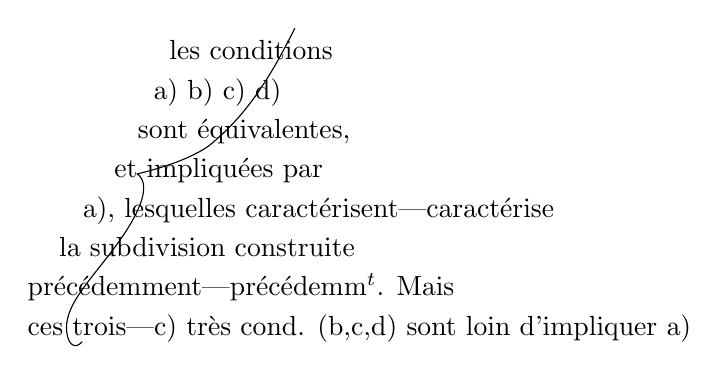
\begin{tikzpicture}[x=1mm,y=1mm,
 every node/.style={anchor=base west,inner sep=0pt}]
 \node at (18,0) {les conditions};
 \node at (16,-5) {\deleted{\unsure{a)}} b) c) d)};
 \node at (14,-10) {sont équivalentes,};
 \node at (11,-15) {\unsure{et} \uline{impliquées} par};
 \node at (7,-20) {a), lesquelles \unsure{caractérisent|caractérise}};
 \node at (4,-25) {la subdivision construite};
 \node at (0,-30) {\unsure{précédemment|précédemm$^{t}$}. Mais};
 \node at (0,-35) {\unsure{ces trois|c) très} \unsure{cond.} (b,c,d) \unsure{sont} \unsure{loin} d'impliquer a)};
 \draw (34,4)
  .. controls (31,-2) and (28,-7) .. (23,-11)
  .. controls (20,-13) and (16,-14) .. (14,-14.5)
  .. controls (16,-16) and (14,-20) .. (11,-24)
  .. controls (8,-28) and (5,-31) .. (5,-34)
  .. controls (5,-36) and (6,-37) .. (7,-35.8);
\end{tikzpicture}}}
